\subsection{Caso d'uso UC10: Modalità allenamento}
\label{UC10}
	\begin{figure}
	\centering
	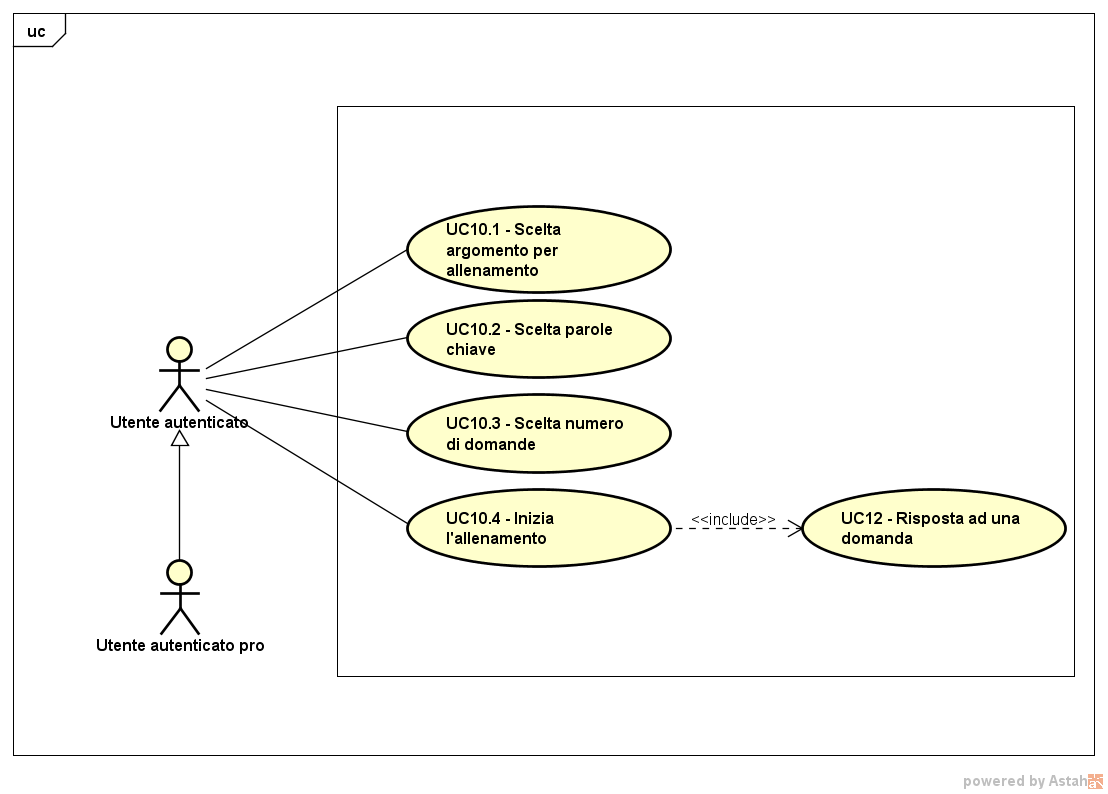
\includegraphics[scale=0.5]{UML/UC10.png}
	\caption{UC10: Modalità allenamento}
	\end{figure}
\FloatBarrier
\begin{itemize}
\item\textbf{Attori}: Utente autenticato, Utente autenticato pro;
\item\textbf{Descrizione}: gli attori possono svolgere un allenamento che consiste nel rispondere a domande che gli vengono proposte in modo dinamico. Ogni domanda può incrementare o decrementare il punteggio dell'allenamento per fare in modo che la difficoltà delle domande proposte sia sempre in linea con la competenza dell'utente sull'argomento scelto;
\item\textbf{Precondizione}: gli utenti hanno selezionato l'opzione di allenamento;
\item\textbf{Postcondizione}: gli attori hanno finito di svolgere l'allenamento e può quindi visualizzare la valutazione finale che ha ottenuto e il riepilogo delle risposte date nonché il proprio livello sugli argomenti;
\item\textbf{Scenario principale}:
	\begin{enumerate}
		\item Gli attori scelgono l'argomento per iniziare l'allenamento (UC10.1);
		\item Gli attori scelgono delle parole chiave (UC10.2);
		\item Gli attori scelgono il numero di domande che compongono l'allenamento (UC10.3);
		\item Gli attori iniziano l'allenamento (UC10.4).
	\end{enumerate}
\item \textbf{Inclusione}:
	\begin{itemize}
		\item Gli attori rispondono ad una domanda (UC12).
	\end{itemize}
\end{itemize}

\subsubsection{Caso d'uso UC10.1: Scelta argomento per l'allenamento}
	\begin{itemize}
		\item \textbf{Attori}: utente autenticato, utente autenticato pro;
		\item \textbf{Descrizione}: gli attori scelgono un macro argomento per eseguire un allenamento;
		\item \textbf{Precondizione}: gli attori scelgono di eseguire un allenamento;
		\item \textbf{Postcondizione}: gli attori hanno scelto un macro argomento per l'allenamento.
	\end{itemize}
\subsubsection{Caso d'uso UC10.2: Scelta parole chiave}
	\begin{itemize}
		\item \textbf{Attori}: utente autenticato, utente autenticato pro;
		\item \textbf{Descrizione}: gli attori scelgono delle parole chiave per filtrare in modo più dettagliato possibile l'argomento delle domande proposte per l'allenamento;
		\item \textbf{Precondizione}: gli attori hanno scelto un argomento;
		\item \textbf{Postcondizione}: gli attori hanno scelto delle parole chiavi.
	\end{itemize}
\subsubsection{Caso d'uso UC10.3: Scelta numero di domande}
	\begin{itemize}
		\item \textbf{Attori}: utente autenticato, utente autenticato pro;
		\item \textbf{Descrizione}: gli attori scelgono il numero di domande che comporranno l'allenamento, senza restrizione sul numero e ipoteticamente anche infinito;
		\item \textbf{Precondizione}: gli attori hanno scelto un argomento e scelto delle parole chiavi;
		\item \textbf{Postcondizione}: gli attori hanno scelto il numero di domande che comporranno l'allenamento.
	\end{itemize}
\subsubsection{Caso d'uso UC10.4: Inizia allenamento}
\label{UC10.4}
\begin{figure}
	\centering
	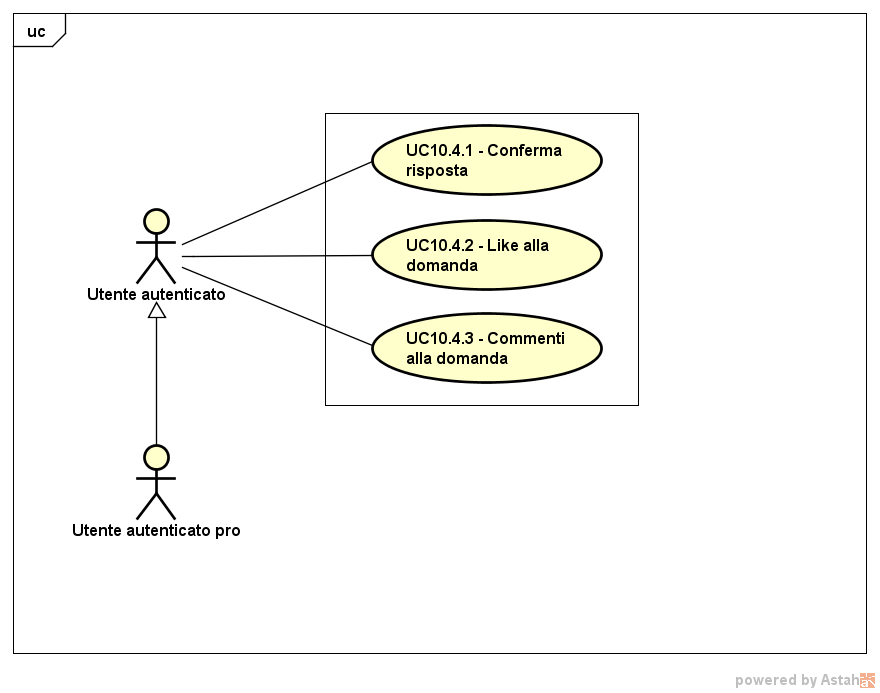
\includegraphics[scale=0.5]{UML/UC10_4.png}
	\caption{UC10.4: Inizia allenamento}
\end{figure}
\FloatBarrier
	\begin{itemize}
		\item \textbf{Attori}: utente autenticato, utente autenticato pro;
		\item \textbf{Descrizione}: gli attori iniziano l'allenamento;
		\item \textbf{Precondizione}: gli attori hanno scelto l'argomento, le parole chiave e il numero di domande;
		\item \textbf{Postcondizione}: gli attori hanno iniziato l'allenamento.
	\end{itemize}
\subsubsection{Caso d'uso UC10.4.1: Conferma risposta}
	\begin{itemize}
		\item \textbf{Attori}: utente autenticato, utente autenticato pro;
		\item \textbf{Descrizione}: gli attori confermano la risposta data;
		\item \textbf{Precondizione}: gli attori hanno risposto ad una domanda;
		\item \textbf{Postcondizione}: gli attori hanno confermato la risposta e proseguono l'allenamento.
	\end{itemize}
\subsubsection{Caso d'uso UC10.4.2: Like alla domanda}
	\begin{itemize}
		\item \textbf{Attori}: utente autenticato, utente autenticato pro;
		\item \textbf{Descrizione}: gli attori possono lasciare un like a una domanda proposta;
		\item \textbf{Precondizione}: agli attori è stata proposta una domanda;
		\item \textbf{Postcondizione}: gli attori hanno rilasciato un like alla domanda proposta.
	\end{itemize}
\subsubsection{Caso d'uso UC10.4.3: Commenti alla domanda}
\label{UC10.4.3}
\begin{figure}
	\centering
	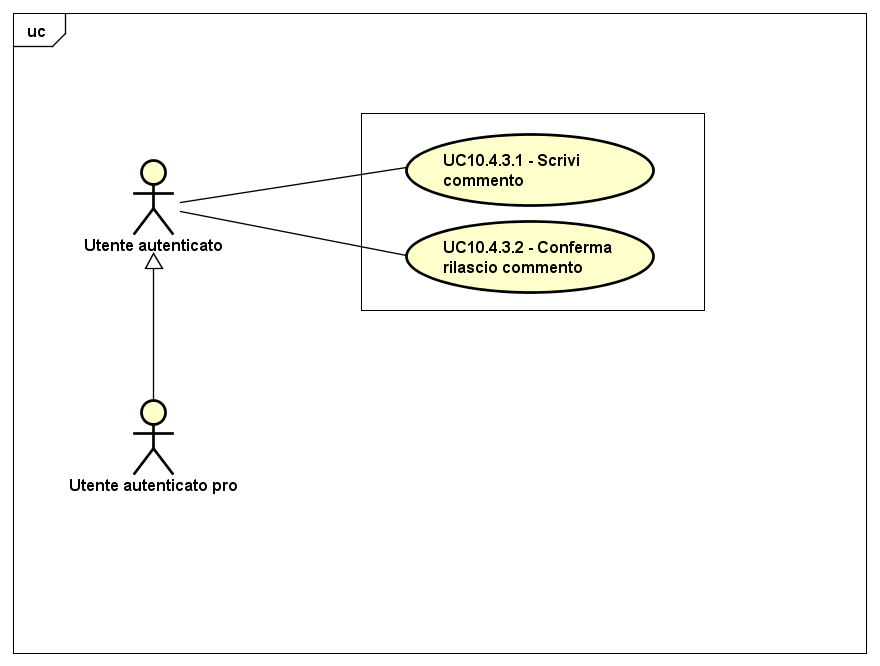
\includegraphics[scale=0.5]{UML/UC10_4_3.png}
	\caption{UC10.4.3: Commenti alla domanda}
\end{figure}
	\begin{itemize}
		\item \textbf{Attori}: utente autenticato, utente autenticato pro;
		\item \textbf{Descrizione}: gli attori possono scegliere di commentare una domanda;
		\item \textbf{Precondizione}: gli attori hanno risposto ad una domanda e visualizzano una sezione per i commenti;
		\item \textbf{Postcondizione}: gli attori hanno scelto di commentare la domanda proposta.
		\item \textbf{Scenario principale}:
			\begin{enumerate}
				\item Gli attori scrivono un commento sulla domanda (UC10.4.3.1);
				\item Gli attori confermano il rilascio del commento (UC10.4.3.2);
			\end{enumerate}
	\end{itemize}
\subsubsection{Caso d'uso UC10.4.3.1: Scrivi commento}
	\begin{itemize}
		\item \textbf{Attori}: utente autenticato, utente autenticato pro;
		\item \textbf{Descrizione}: gli attori possono scrivere il commento alla domanda proposta;
		\item \textbf{Precondizione}: gli attori hanno scelto di scrivere un commento;
		\item \textbf{Postcondizione}: gli attori hanno scritto un commento.
	\end{itemize}
\subsubsection{Caso d'uso UC10.4.3.2: Conferma rilascio commento}
	\begin{itemize}
		\item \textbf{Attori}: utente autenticato, utente autenticato pro;
		\item \textbf{Descrizione}: gli attori possono confermare il rilascio del commento scritto;
		\item \textbf{Precondizione}: gli attori hanno scritto un commento;
		\item \textbf{Postcondizione}: gli attori hanno commentato una domanda.
	\end{itemize}
\subsubsection{Caso d'uso UC10.4.4: Segnalare la domanda}
\label{UC10.4.4}
\begin{figure}
	\centering
	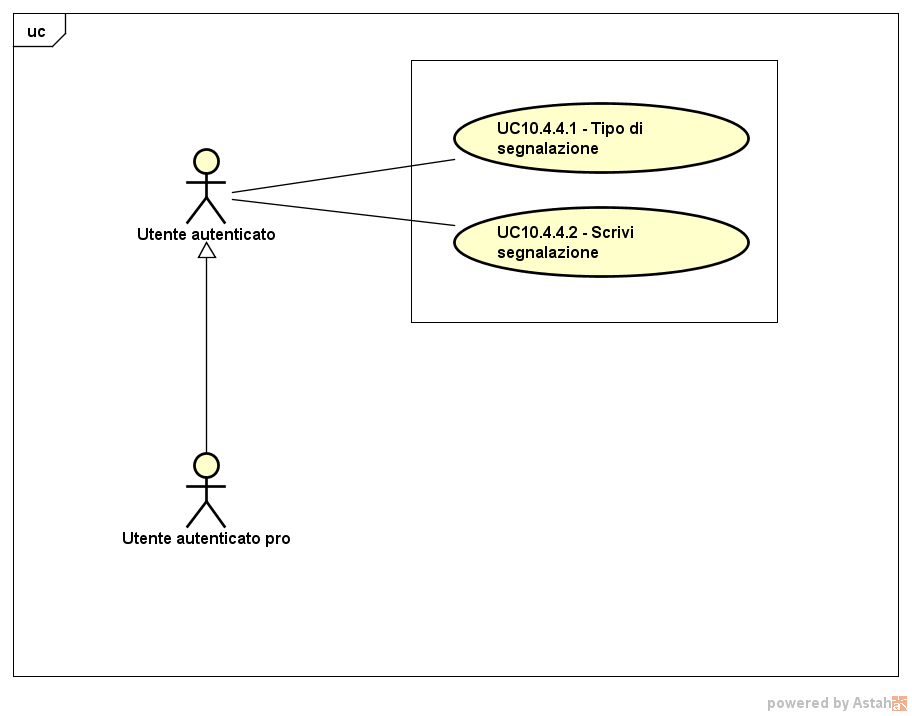
\includegraphics[scale=0.5]{UML/UC10_4_4.png}
	\caption{UC10.4.4: Segnalare una domanda}
\end{figure}
\FloatBarrier
	\begin{itemize}
		\item \textbf{Attori}: utente autenticato, utente autenticato pro;
		\item \textbf{Descrizione}: gli attori possono segnalare una domanda se ritengono che sia sbagliata, mal formata oppure contenga contenuti non appropriati;
		\item \textbf{Precondizione}: gli attori hanno visualizzato il resoconto dell'allenamento;
		\item \textbf{Postcondizione}: gli attori hanno scelto di segnalare una domanda;
				\item \textbf{Scenario principale}:
				\begin{enumerate}
					\item Gli attori scelgono il tipo di segnalazione tra quelli proposti (UC10.4.4.1);
					\item Gli attori scrivono il contenuto della segnalazione (UC10.4.4.2);
				\end{enumerate}
	\end{itemize}
\subsubsection{Caso d'uso UC10.4.4.1: Tipo di segnalazione}
	\begin{itemize}
		\item \textbf{Attori}: utente autenticato, utente autenticato pro;
		\item \textbf{Descrizione}: gli attori possono decidere il tipo di segnalazione tra quelli proposti;
		\item \textbf{Precondizione}: gli attori hanno scelto di segnalare una domanda;
		\item \textbf{Postcondizione}: gli attori hanno scelto il tipo di segnalazione.
	\end{itemize}
\subsubsection{Caso d'uso UC10.4.4.2: Scrivi segnalazione}
	\begin{itemize}
		\item \textbf{Attori}: utente autenticato, utente autenticato pro;
		\item \textbf{Descrizione}: gli attori posso scrivere un commento sulla segnalazione per approfondire la motivazione;
		\item \textbf{Precondizione}: gli attori hanno scelto di segnalare una domanda;
		\item \textbf{Postcondizione}: gli attori hanno segnalato una domanda.
	\end{itemize}
\subsubsection{Caso d'uso UC10.4.5: Avanzamento domanda successiva}
	\begin{itemize}
		\item \textbf{Attori}: utente autenticato, utente autenticato pro;
		\item \textbf{Descrizione}: gli attori possono avanzare alla domanda successiva dopo aver risposto alla domanda proposta; 
		\item \textbf{Precondizione}: gli attori hanno risposto alla domanda proposta;
		\item \textbf{Postcondizione}: gli attori visualizzano la domanda successiva.
	\end{itemize}
\subsubsection{Caso d'uso UC10.4.6: Conclusione allenamento}
	\begin{itemize}
		\item \textbf{Attori}: utente autenticato, utente autenticato pro;
		\item \textbf{Descrizione}: gli attori possono concludere l'allenamento in qualunque punto dell'allenamento;
		\item \textbf{Precondizione}: gli attori stanno eseguendo un allenamento;
		\item \textbf{Postcondizione}: gli attori hanno concluso l'allenamento e visualizzano il risultato finale e le statistiche.
	\end{itemize}